\begin{figure}[htbp]
    \centering
    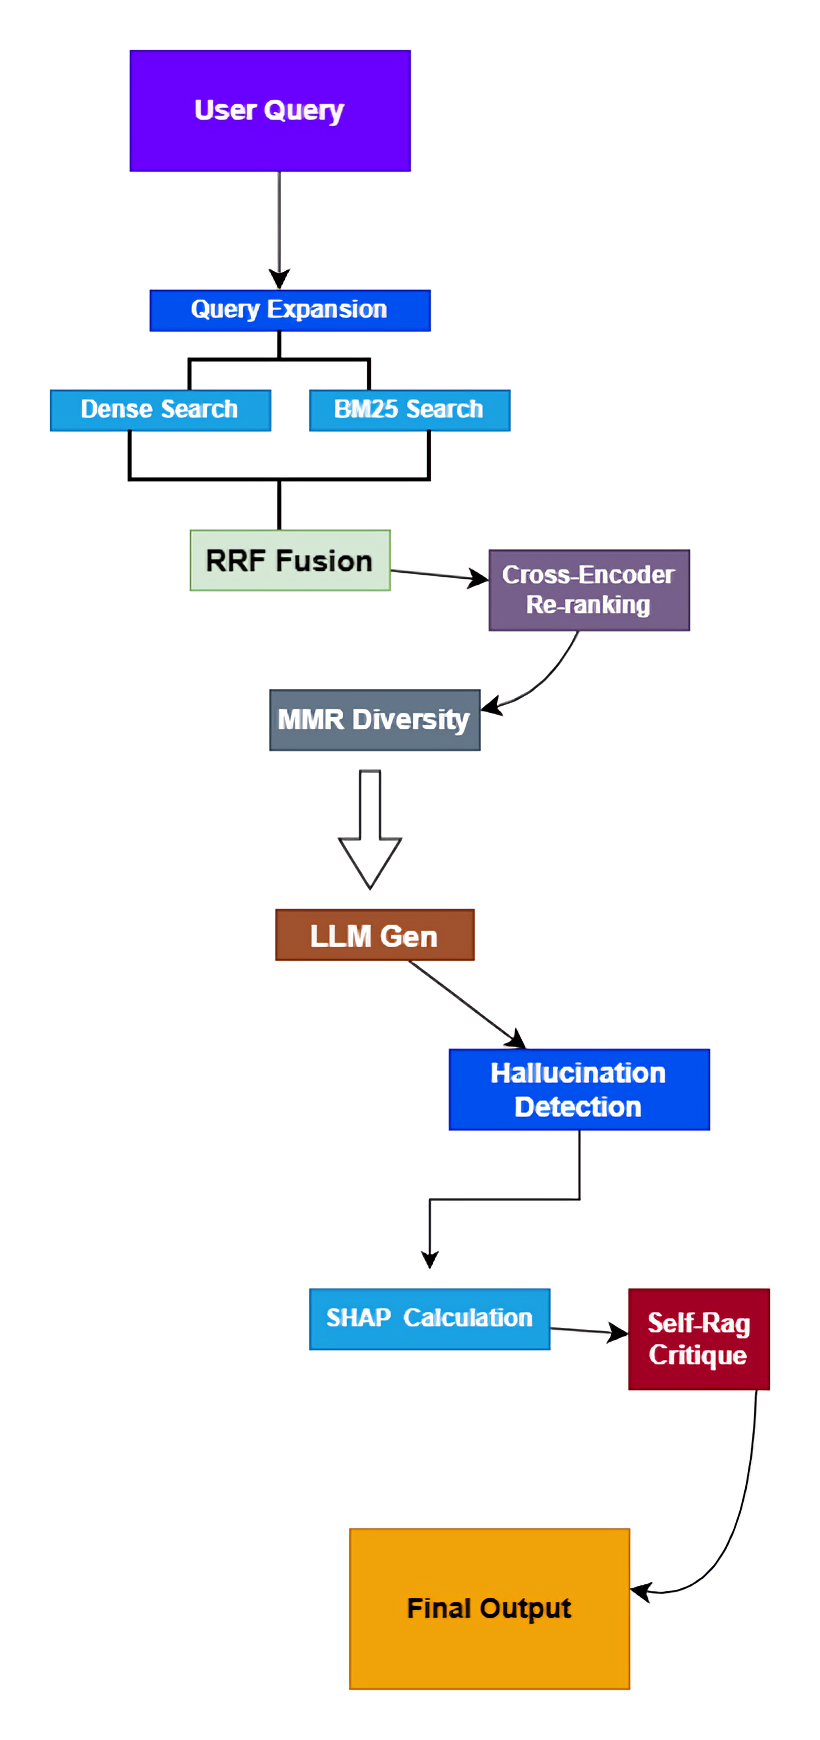
\includegraphics[width=1.0\textwidth, height=0.7\textheight, keepaspectratio]{images/Untitled Diagram.drawio (5) (2).png}
    \caption{Model Architecture Diagram}
    \label{fig:trustrag_architecture}
\end{figure}
\section{Design Process or Methodology Overview}
The framework is organised into five functional blocks, mapped onto the detailed architecture of Fig.~1.2: hybrid graph-aware retrieval, a causal knowledge-graph encoder, a latent world model, calibrated uncertainty, and Shapley source tracking. This section specifies each block and the training objectives.

\subsection{Hybrid Graph-Aware Retrieval}

Given a query $q$, HyDE generates $n_h = 3$ hypothetical sub-answers that are embedded and averaged to form an expanded query representation. We retrieve with a dense MiniLM bi-encoder over a FAISS index and with BM25, and fuse the two ranked lists by reciprocal rank fusion (RRF).

\begin{equation}
\mathrm{RRF}(d)=\sum_{r\in\{\mathrm{dense,bm25}\}}
\frac{1}{k+\mathrm{rank}_r(d)},
\qquad k=60
\end{equation}

A cross-encoder re-scores the top candidates, and maximal marginal relevance (MMR) selects a final set that balances relevance and diversity:

\begin{equation}
\mathrm{MMR}=
\arg\max_{d\in R\setminus S}
\left[
\lambda\,\mathrm{rel}(d,q)
-(1-\lambda)\max_{d'\in S}\mathrm{sim}(d,d')
\right]
\end{equation}

with $\lambda=0.6$.

\subsection{Causal Knowledge-Graph Encoder}

A medical knowledge graph with $N=20$ nodes encodes a sparse stochastic causal prior over symptom--pathology relations. An edge-biased graph attention network processes the graph. The attention logits are:

\begin{equation}
\alpha_{ij}^{(h)}
\propto
\frac{
(W_qx_i)^T(W_kx_j)
}
{\sqrt{d_h}}
+
W_e e_{ij}
\end{equation}

A masked mean pool yields a graph embedding $g\in\mathbb{R}^{256}$.

\subsection{Latent World Model}

The core contribution is an action-conditioned latent dynamics model. At each step, a causal residual computes the effect of action $a_t$ on the latent state:

\begin{equation}
\Delta z_t
=
s\cdot
\sigma
\left(
W_g[z_t,h]
\right)
\odot
\mathrm{MLP}
\left(
[z_t,g,e_{a_t}]
\right)
\end{equation}

The next latent state is predicted by:

\begin{equation}
z_{t+1}
=
h2z
\left(
\mathrm{GRU}
\left(
[z_t+\Delta z_t,e_{a_t}]
\right)
\right)
\end{equation}

\subsection{Tree-of-Thought Beam Planner}

Plan selection is formulated as a beam-search process using the world model as the transition function.

\begin{equation}
J(\pi)
=
v_{\theta}(z_H)
+
\beta
\sum_t
r_{\phi}(z_t,z_{t+1})
-
\gamma
\bar{\sigma}(z_H)
\end{equation}

where $\beta=0.5$ and $\gamma=0.1$.

\subsection{Deep-Ensemble Uncertainty}

Five probabilistic ensemble heads emit Gaussian predictions and uncertainties:

\begin{equation}
\mu
=
\frac{1}{M}
\sum_m \mu_m
\end{equation}

\begin{equation}
\sigma^2_{\text{total}}
=
\underbrace{\mathrm{Var}_m(\mu_m)}_{\text{epistemic}}
+
\underbrace{
\frac{1}{M}
\sum_m \sigma_m^2
}_{\text{aleatoric}}
\end{equation}

\subsection{Shapley Source Tracking}

Original-source tracking attributes answer quality to each retrieved document using Shapley values:

\begin{equation}
\phi_i
=
\mathbb{E}_{\pi}
\left[
v(S_i^{\pi}\cup\{i\})
-
v(S_i^{\pi})
\right]
\end{equation}

where $v(\cdot)$ denotes the subset relevance score.

\subsection{Training Objectives}

The world model minimises:

\begin{equation}
L_{wm}
=
\|\hat{o}-o\|^2
+
0.01\|\Delta z\|^2
+
0.001\bar{\sigma}
+
0.1\|r_{\phi}-r^{*}\|^2
\end{equation}

The ensemble is trained using Gaussian negative log-likelihood:

\begin{equation}
L_{ens}
=
\frac{1}{M}
\sum_m
\frac{1}{2}
\left(
\log\sigma_m^2
+
\frac{(y-\mu_m)^2}{\sigma_m^2}
\right)
\end{equation}

\begin{table}[H]
\centering
\caption{Key hyperparameters.}
\label{tab:hyperparameters}
\begin{tabular}{|l|l|c|}
\hline
\textbf{Group} & \textbf{Parameter} & \textbf{Value} \\
\hline
Architecture & Latent / Hidden Dimension & 256 / 512 \\
Architecture & Transformer Layers / Heads & 3 / 8 \\
Architecture & GNN Layers & 3 \\
Architecture & Ensemble Members & 5 \\
Planning & Beam Width / Depth & 8 / 4 \\
Planning & Reward Weight $\beta$ & 0.5 \\
Planning & Uncertainty Penalty $\gamma$ & 0.1 \\
Retrieval & Top-k / Embedding Dimension & 6 / 384 \\
Retrieval & MMR $\lambda$ / RRF $k$ & 0.6 / 60 \\
Retrieval & HyDE Sub-Queries & 3 \\
Retrieval & SHAP Permutations & 32 \\
Optimisation & WM / Ensemble Epochs & 15 / 10 \\
Optimisation & WM / Ensemble Learning Rate & $2\times10^{-4}$ / $10^{-3}$ \\
Optimisation & Batch Size / Precision & 64 / FP16 \\
\hline
\end{tabular}
\end{table}
 
\textbf{Key Observation:}
It was found that behavioral priori authentication using dynamic authentication and behavioral biometrics was not compatible with class models with experimentation and design. They would also probably need to retrain all new users heavily and therefore interfere with personalization. Nonetheless, the Siamese model was highly scalable so that comparisons without learning classes could be made directly. It is believed that LSTM is a more suitable alternative when modeling swipes, holds and typing rhythms as, although computationally tractable, the GRU-based models frequently could not map out all relationships of behavioral complexity in longer sequence interactions.
The system, as it interprets and defines decisions in the same way with a certain threshold of similarity being 65 percent managed to be rather practical. This combination was an effective solution to the verification of behavioral biometrics because this would resolve the issue of achieving per-user authentication in addition to providing a high level of security with the minimal user input.

\section{Data Collection -}
We take three public sources and assemble100,000 samples (Table4.2). DDXPlus [22] supplies
MedMCQA[23] items become the retrievable patient records, while world model dynamics are driven by patient records.
The held-out evaluation queries come from MedQA-USMLE[24] and evidence corpus is available. All three are
Fetched or downloaded from public mirrors, stored locally without authentication.

\begin{table}[H]
\centering
\caption{Dataset composition (100,000 samples).}
\label{tab:dataset}
\begin{tabular}{l l r}
\hline
\textbf{Dataset} & \textbf{Role} & \textbf{Size} \\
\hline
DDXPlus (train/val/test) & World-model dynamics & 80k/10k/10k \\
MedMCQA & Evidence corpus & 50,000 docs \\
MedQA-USMLE & Held-out evaluation & 1,000 queries \\
\hline
\end{tabular}
\end{table}


\subsection{Data Cleaning}
All DDXPlus records are parsed and validated prior to use. audit mising training split
Labels on the pathology—Empty differential diagnoses—Empty evidence lists—Parse failures of the
string-encoded list fields. 0.9997 of all 80,000 training records satisfy these completeness testing (Fig.~\ref{fig:cleaning}a),
Note that it is not necessary to delete records, only to format the curated source.
The cleaned distributions were evaluated using exploratory analysis (Fig.~\ref{fig:eda}) which revealed that  patient age is widely distributed.
The age split at diagnosis (mean 39.6, standard deviation 22.7years) is almost equal (0.486 male, 0.514 female)
Female patients are predominately affected by upper respiratory and viral conditions, while the pathology distribution is led for the male gender by upper respiratory and bacterial conditions.
The median number of clinical evidence carried by each is 19.


\begin{figure}[H]
\centering
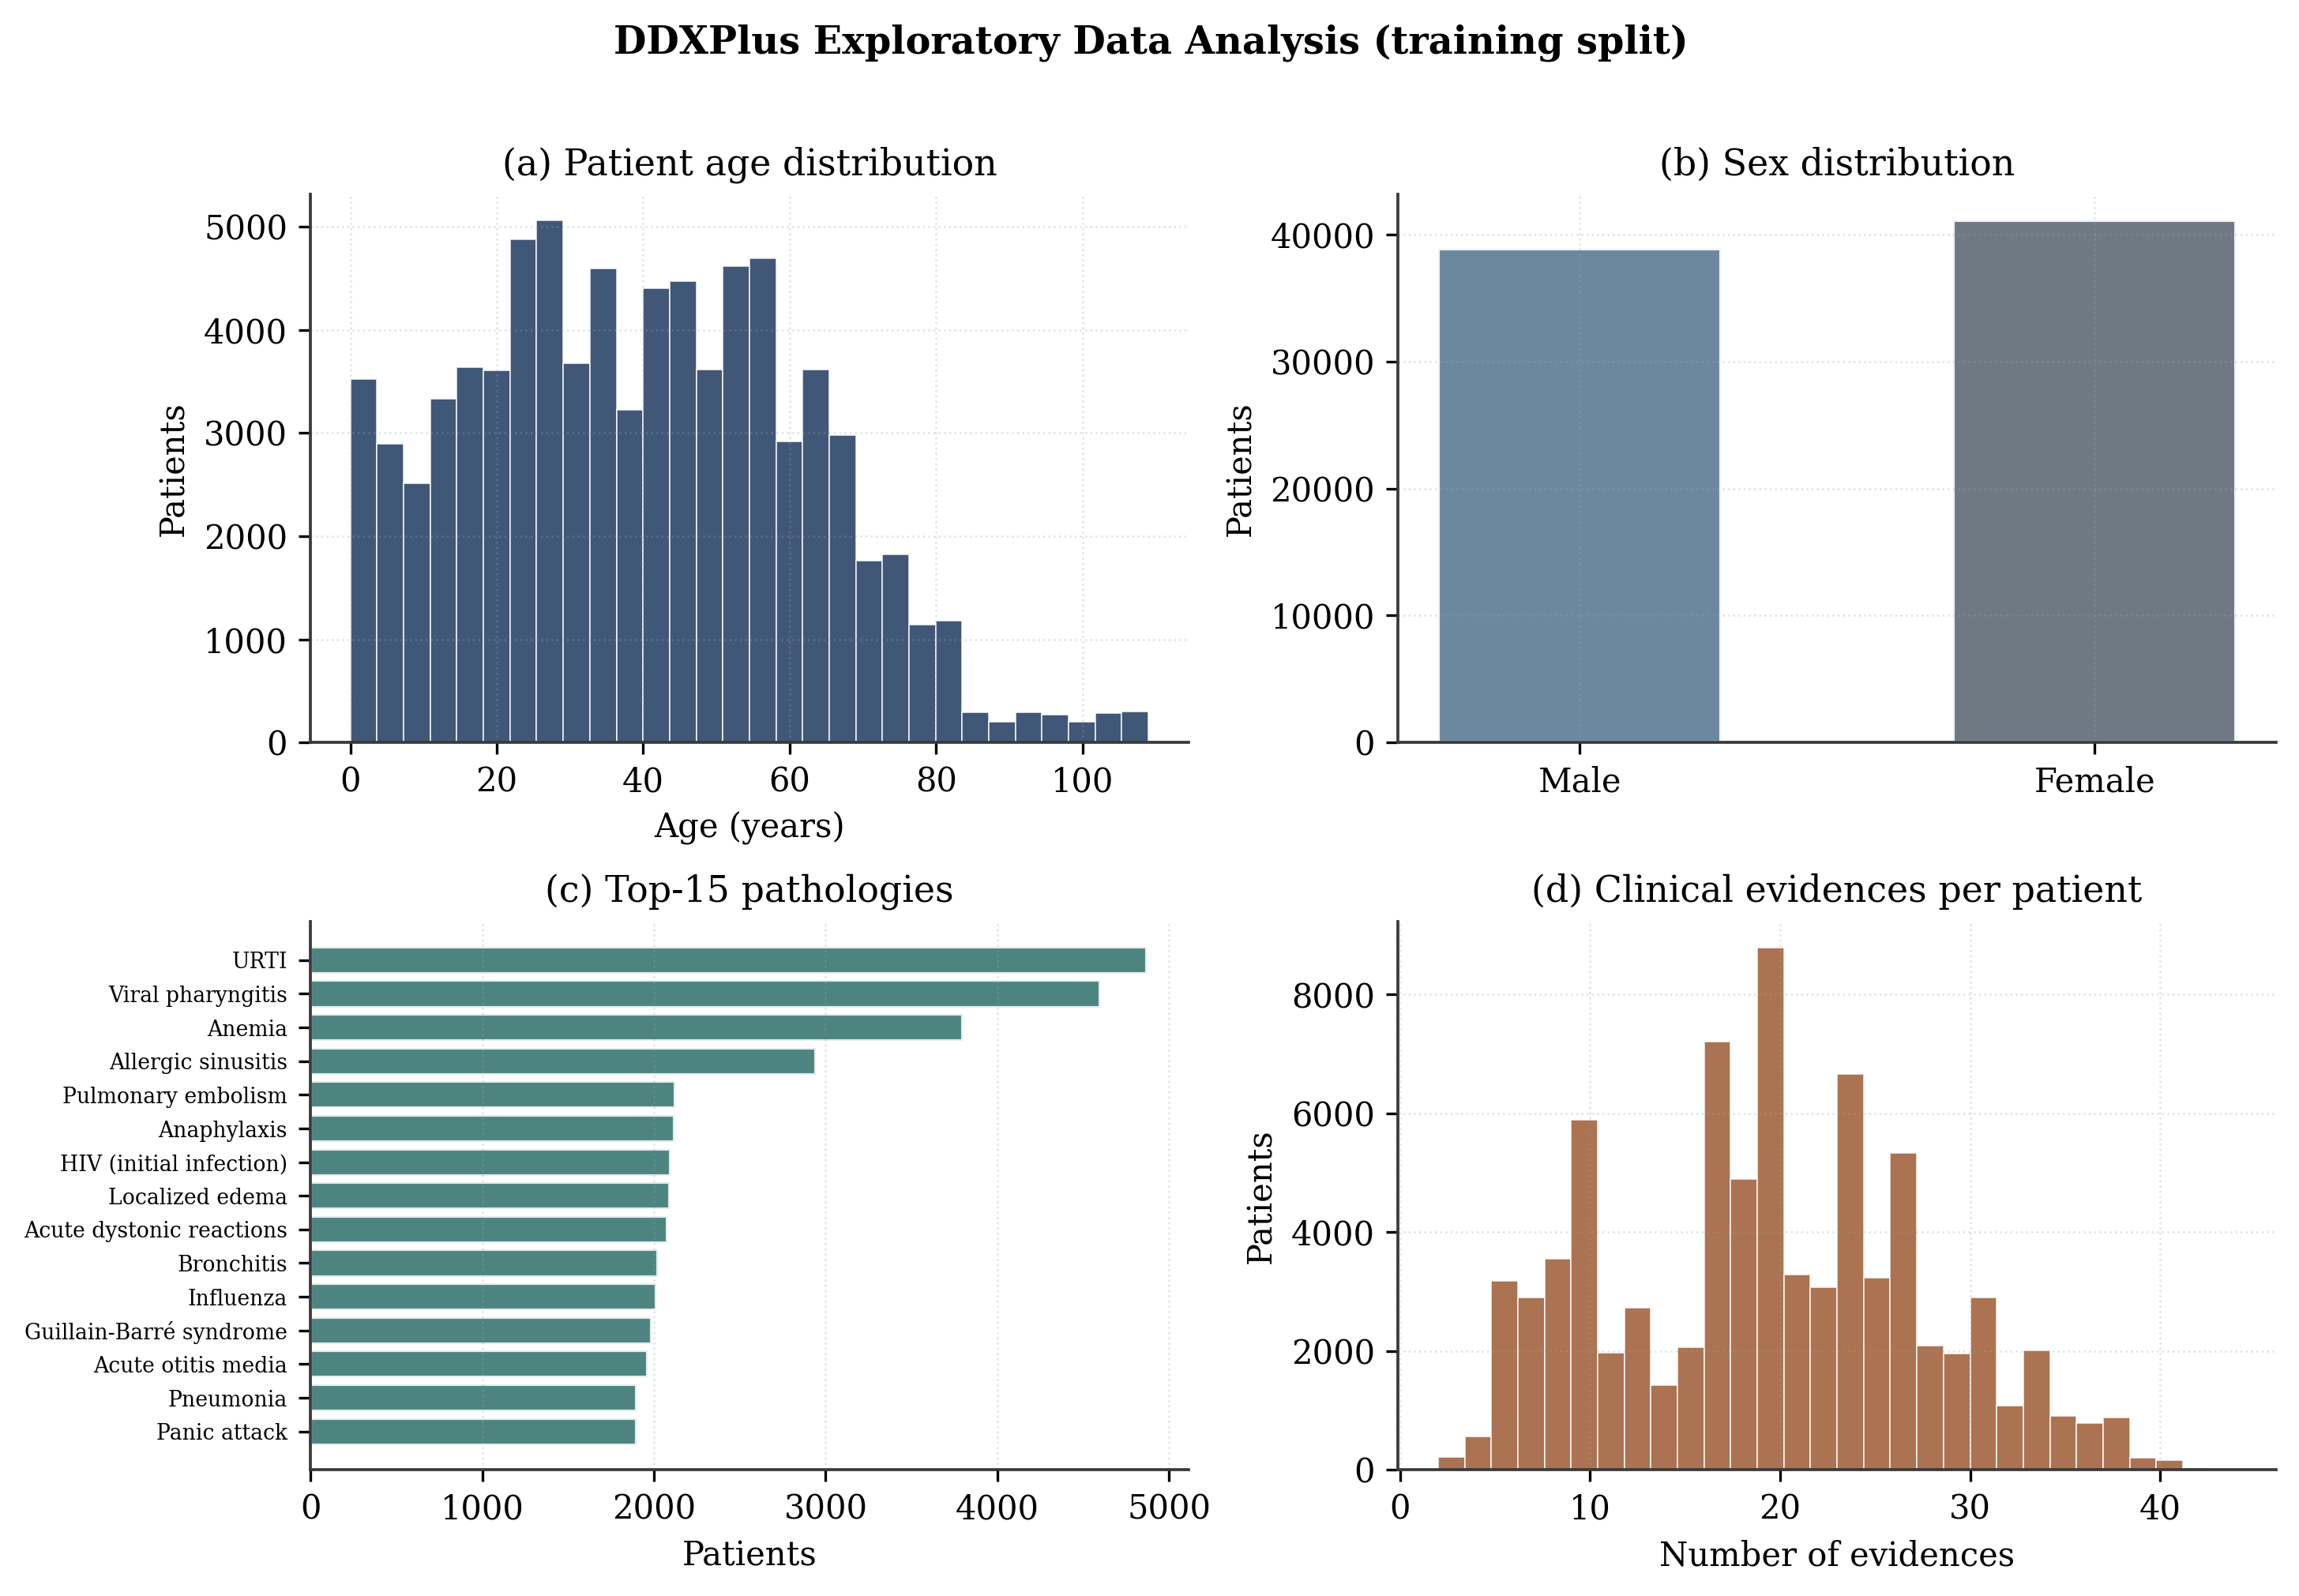
\includegraphics[width=\textwidth,keepaspectratio]{images/fig13_data_overview.png}
\caption{Exploratory data analysis of the cleaned DDXPlus training split: (a) patient age distribution; (b) sex distribution; (c) the fifteen most frequent pathologies; and (d) the number of clinical evidences per patient.}
\label{fig:eda}
\end{figure}

\begin{figure}[H]
\centering
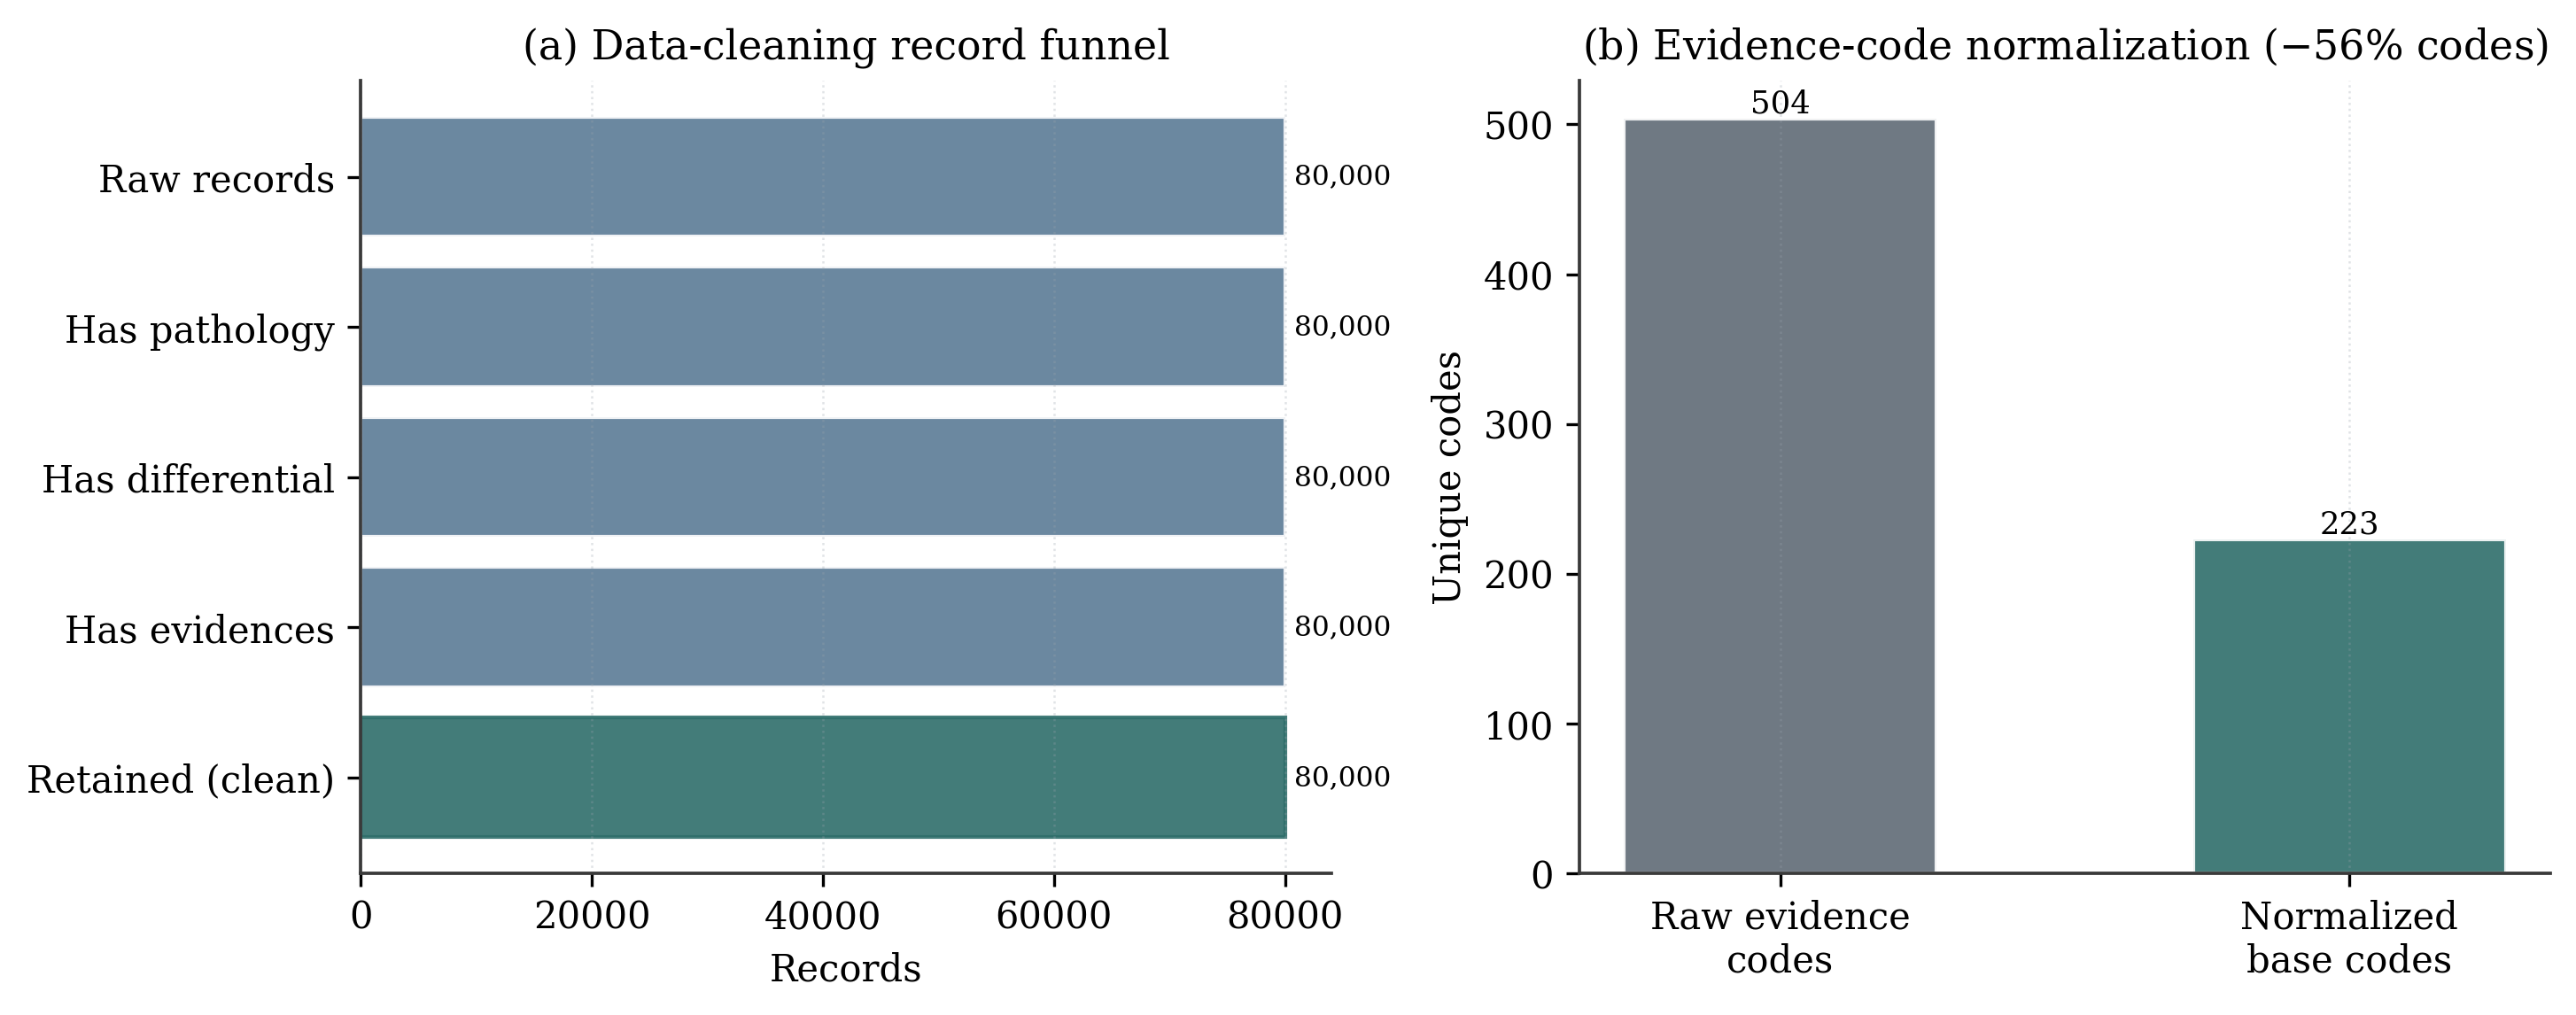
\includegraphics[width=\textwidth,keepaspectratio]{images/fig14_data_cleaning.png}
\caption{Data cleaning. (a) Record-level validation funnel: all 80,000 training records satisfy the completeness checks. (b) Evidence-code normalisation collapses 504 raw, value-suffixed codes to 223 canonical base codes, reducing sparsity before encoding.}
\label{fig:cleaning}
\end{figure}






\subsection{Data Transformation}

The cleaned records are now in model form. The evidence codes for raw evidence are of the form
\[
E_{54\_@\_V\_{161}}
\]
and are normalised to canonical base codes ($E_{54}$), reducing the unique-code vocabulary from 504 to 223 (Fig.~\ref{fig:cleaning}b) and removing value-suffix sparsity. Age is scaled to the interval $[0,1]$, sex is represented by a binary indicator, and the evidence set is represented by binary flags.

Each patient trajectory is modelled as an 8-step diagnostic sequence, where evidence is made available one item at a time while being represented over 64 dimensions. At each step, there is a discrete action corresponding to acquiring evidence, and the outcome is represented by a 5-dimensional vector equivalent to the top-$k$ distribution for differential diagnosis.


\subsection{Data Integration}
The three sources are combined in a single pipeline: DDXPlus trajectories train and evaluate
The world model and ensemble: MedMCQA items are embedded and indexed (dense + BM25)
the retrievable evidence corpus that provides context labels and the Shapley attribution pool; and
The end-to-end comparison is spurred by the queries posed by MedQA-USMLE. A common language of 49 diseases
The structured and the textual modalities are connected by and 223 evidence base codes.

\subsection{Data Reduction }
The preprocessing pipeline (Fig.~\ref{fig:prepipe}) compresses high cardinality string-encoded records to compact ones.
Formatting noise is removed by tensors cleaning, transformation in normalisation and encoding, integration in joining.
the sources, and reduction projects each patient into a fixed 64-dimensional observation space.
Having an outcome of 5 dimension. This yields a dense numerical representation which is small enough to
Train in minutes, but rich enough to maintain clinically meaningful structure.


\begin{figure}[H]
\centering
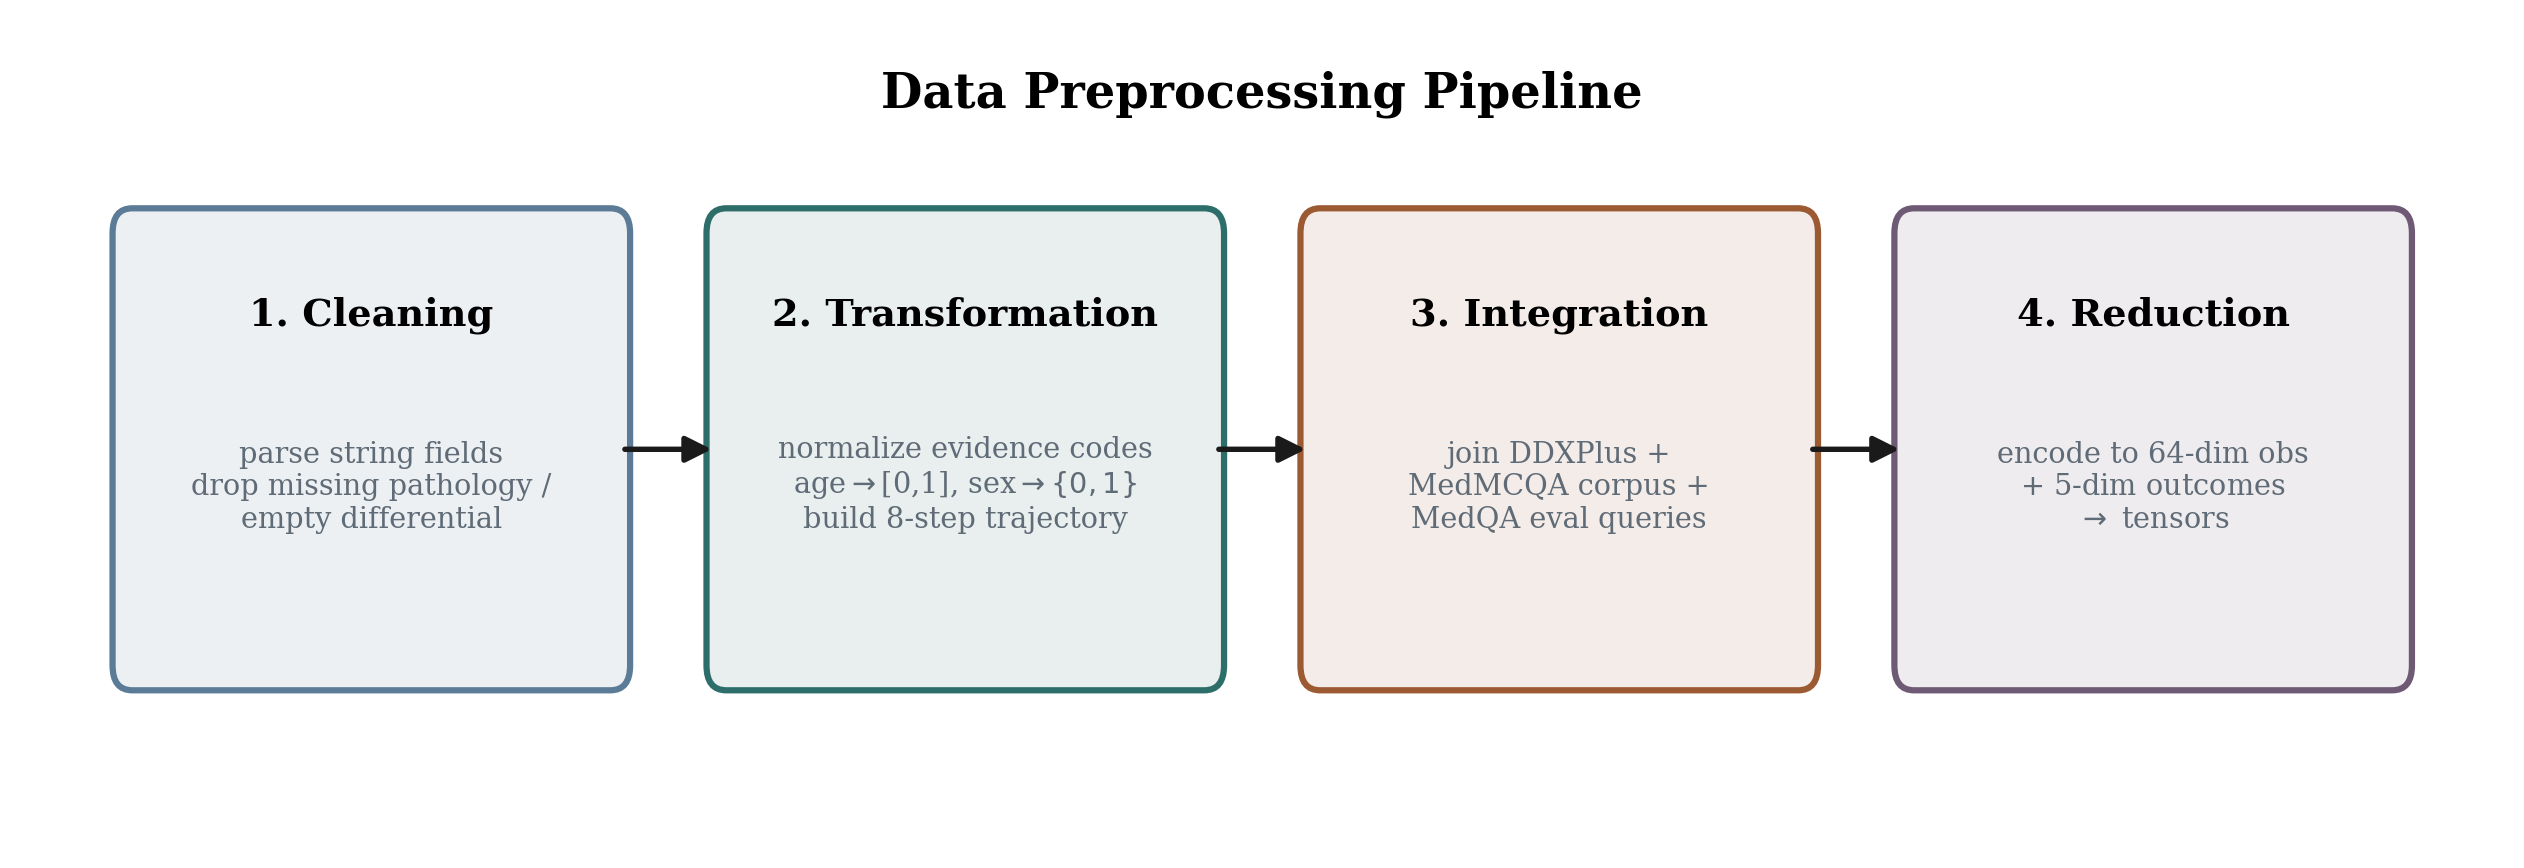
\includegraphics[width=\textwidth,keepaspectratio]{images/fig18_preprocess_pipeline.png}
\caption{Data preprocessing pipeline: cleaning, transformation, integration, and reduction map raw clinical records to fixed-size tensors.}
\label{fig:prepipe}
\end{figure}





\subsection{Summary of Preprocessed Data}
The preprocessed data has two characteristics that influence evaluation. First, the pathology
Its distribution is heavily skew-tailed over 49 classes (Fig.~\ref{fig:classstruct}a) and the true patho is in the topranked patho for the large majority of patients (Fig.~\ref{fig:classstruct}b), hence its distribution is not that of a normal distribution.
It's a challenging metric: rank-based macro-F1. Second, the engineered 64-dimensional observation
Possesses a separate data space for information, dimensions for Age, Sex are almost always active, Evidence dimensions
activate at clinically plausible rates and the evidence co-occurrence structure forms coherent
The encoding captures real symptom correlations (not just the original) as shown in blocks (Fig.~\ref{fig:featspace}),
noise.


\begin{figure}[H]
\centering
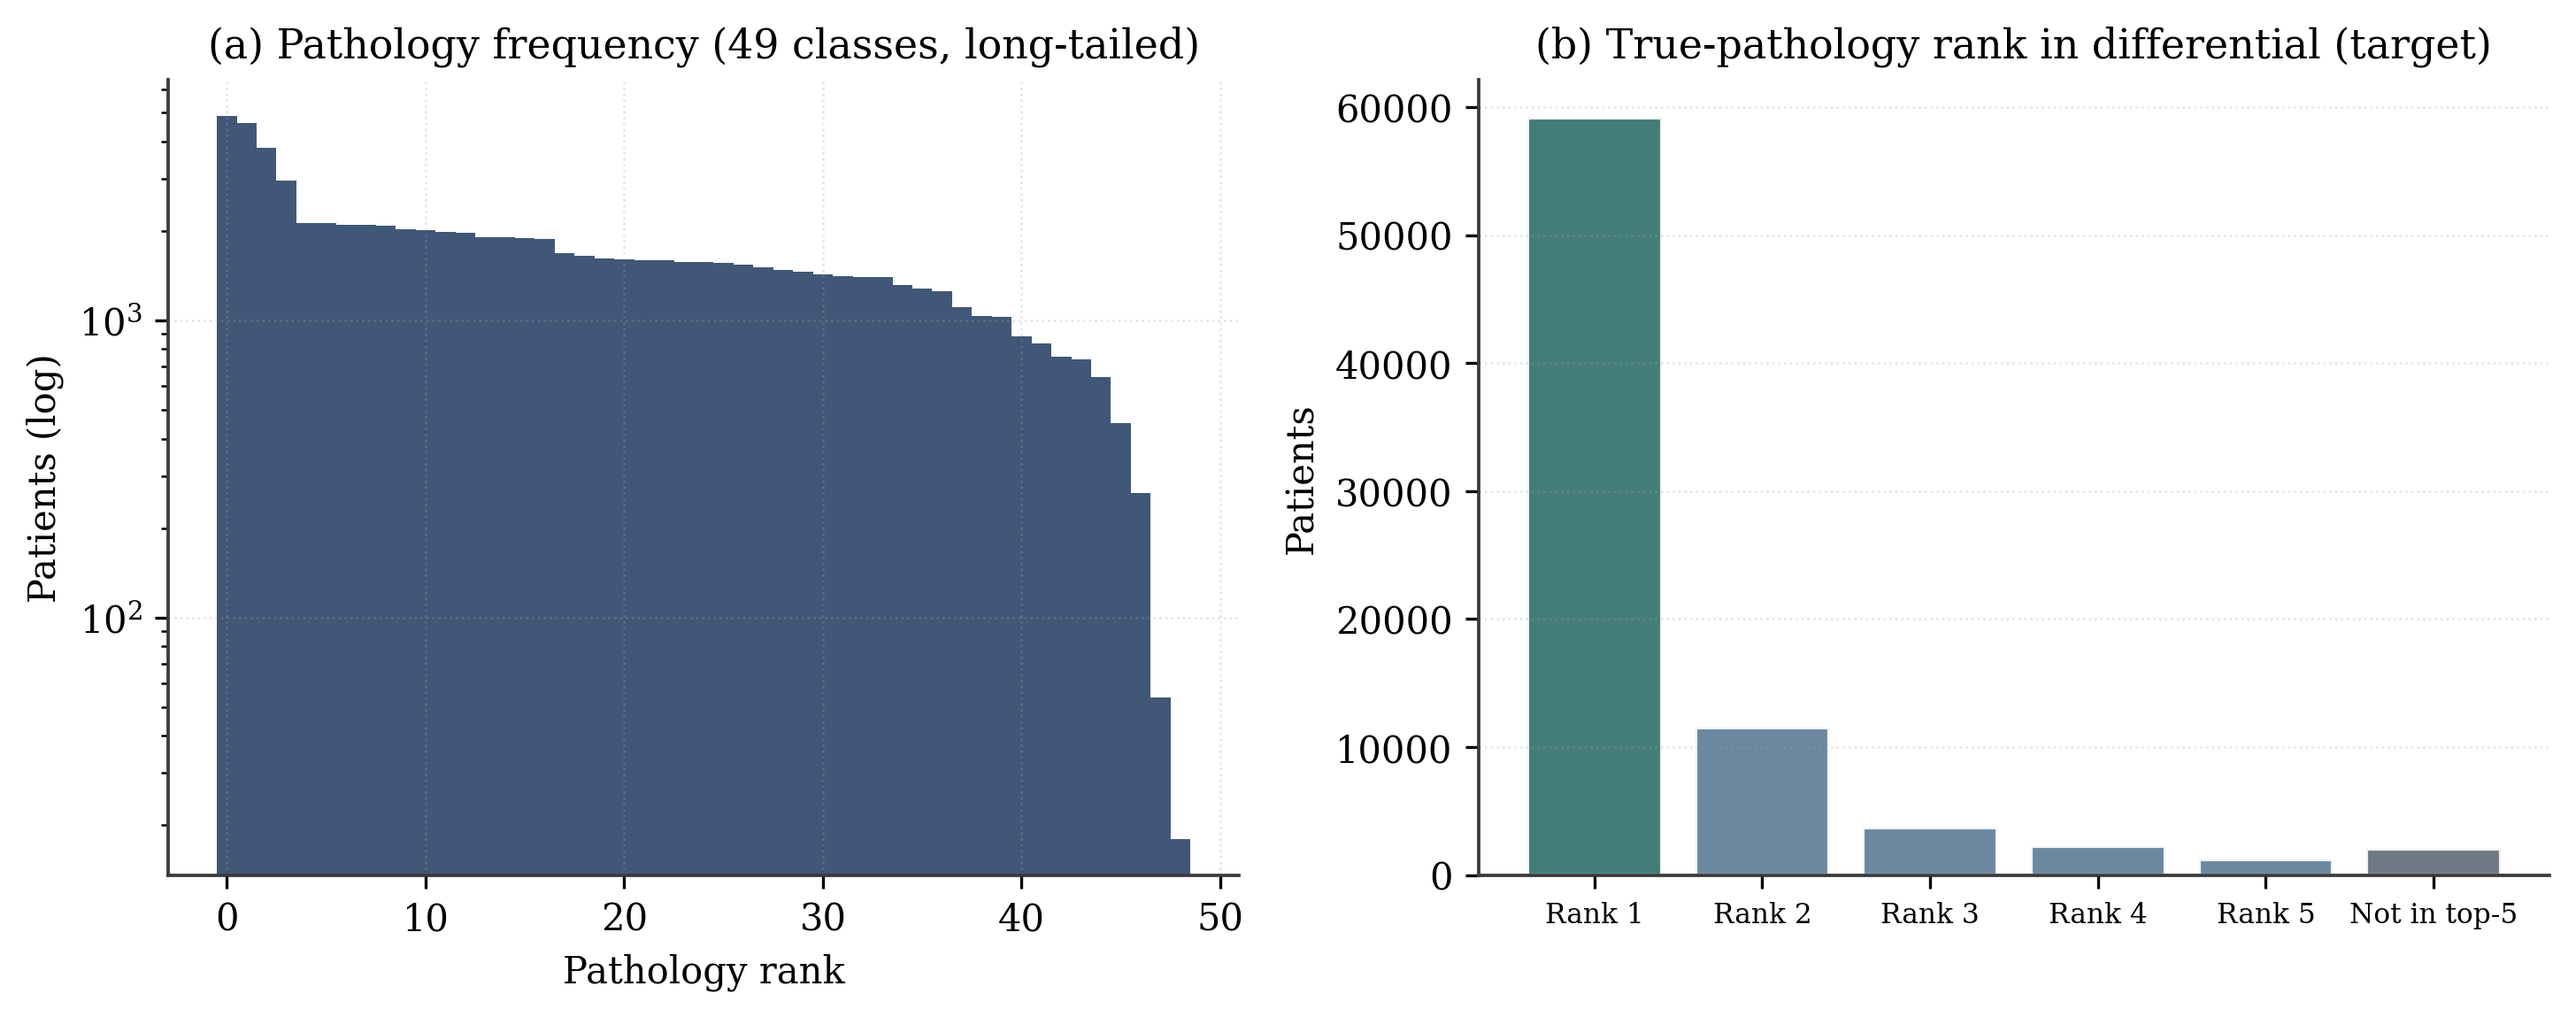
\includegraphics[width=\textwidth,keepaspectratio]{images/fig15_class_imbalance.png}
\caption{Class structure of the preprocessed data. (a) Pathology frequency across 49 classes on a log scale, showing a long tail. (b) Distribution of the true pathology's rank within the differential-diagnosis target.}
\label{fig:classstruct}
\end{figure}

\begin{figure}[H]
\centering
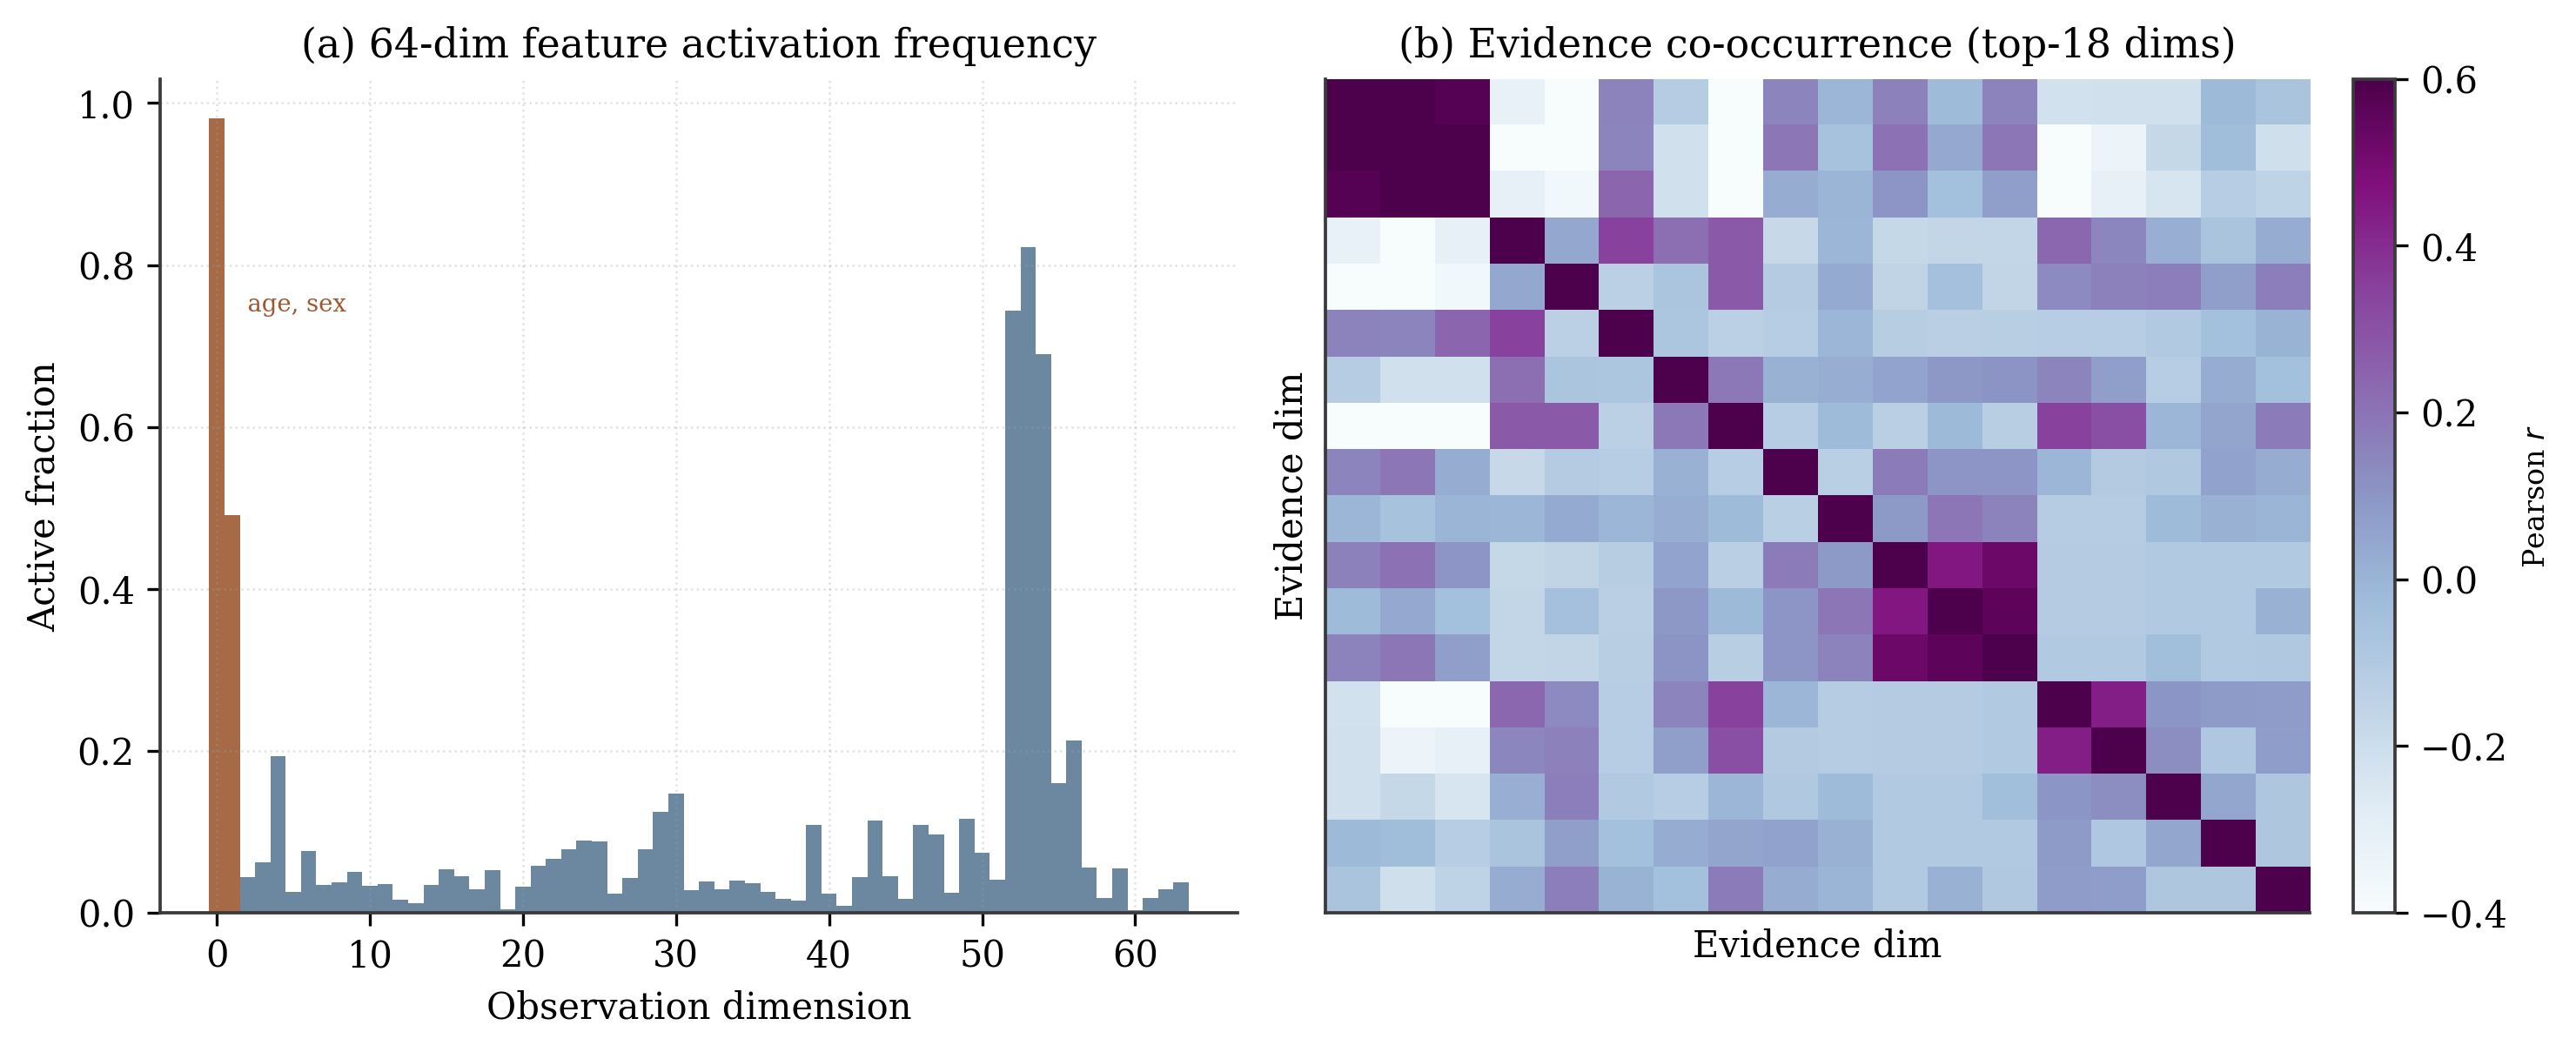
\includegraphics[width=\textwidth,keepaspectratio]{images/fig16_preprocessed_summary.png}
\caption{Preprocessed feature space. (a) Activation frequency of each of the 64 observation dimensions (age and sex highlighted). (b) Pearson co-occurrence among the eighteen most active evidence dimensions, showing coherent clinical blocks.}
\label{fig:featspace}
\end{figure}




